\exercice Placez le point $B$, image du point $A$ par la translation de vecteur~\vectaffiche{u}~+~\vectaffiche{v}.

\begin{tikzpicture}[scale=0.7]
	\placerpoint{A}{0}{0}{below left};
%	Correction
	\placerpointcolor{B}{4}{0}{right}{red};
	\vectAuColor{u}{0}{0}{5}{3}{1pt}{0.5}{above,sloped}{\couleurVect};
	\vectAuColor{v}{5}{3}{-1}{-3}{1pt}{0.5}{above,sloped}{\couleurVect};
	\vectAu{u}{12}{0}{5}{3}{1pt};
	\vectAu{v}{9}{2}{-1}{-3}{1pt};
\end{tikzpicture}

\exercice	\begin{enumerate}
				\item Construisez le point $B$ tel que \vectaffiche{AB} = \vectaffiche{u} + \vectaffiche{v}.
				\item Construisez le point $C$ tel que \vectaffiche{AC} = \vectaffiche{u} + \vectaffiche{v} + \vectaffiche{w}.
				\item Construisez le point $D$ tel que \vectaffiche{AD} = \vectaffiche{u} + \vectaffiche{v} $-$ \vectaffiche{w}.\\
			\end{enumerate}


\begin{tikzpicture}[scale=0.7]
	\placerpoint{A}{0}{0}{below left};
%	Correction
	\placerpointcolor{B}{5}{4}{above left}{\couleurNom};
	\placerpointcolor{C}{4}{2}{below}{\couleurNom};
	\placerpointcolor{D}{6}{6}{above left}{\couleurNom};
	\vectAuColor{u}{0}{0}{10}{3}{1pt}{0.5}{above,sloped}{\couleurVect};
	\vectAuColor{v}{10}{3}{-5}{1}{1pt}{0.5}{above,sloped}{\couleurVect};
	\vectAuColor{w}{5}{4}{-1}{-2}{1pt}{0.5}{below,sloped}{\couleurVect};
	\vectAuColorOppose{w}{5}{4}{1}{2}{1pt}{0.5}{below,sloped}{magenta};
	
	\vectAuColor{AC}{0}{0}{4}{2}{1pt,dotted}{0.7}{,sloped}{magenta};
	\vectAuColor{AB}{0}{0}{5}{4}{1pt,dotted}{0.6}{,sloped}{magenta};
	\vectAuColor{AD}{0}{0}{6}{6}{1pt,dotted}{0.6}{above,sloped}{magenta};

	\vectAu{u}{6}{-2}{10}{3}{1pt};
	\vectAu{v}{4}{5}{-5}{1}{1pt};
	\vectAu{w}{12}{4}{-1}{-2}{1pt};
	\vectAuColorOppose{w}{13}{2}{1}{2}{1pt}{0.5}{above,sloped}{magenta};
\end{tikzpicture}

\newpage

Détail des constructions de chacun des trois points :

\begin{tikzpicture}[scale=0.7]
	\placerpoint{A}{0}{0}{below left};
%	Correction
	\placerpointcolor{B}{5}{4}{above left}{\couleurNom};
%	\placerpointcolor{C}{4}{2}{below}{\couleurNom};
%	\placerpointcolor{D}{6}{6}{above left}{\couleurNom};
	\vectAuColor{u}{0}{0}{10}{3}{1pt}{0.5}{above,sloped}{\couleurVect};
	\vectAuColor{v}{10}{3}{-5}{1}{1pt}{0.5}{above,sloped}{\couleurVect};
%	\vectAuColor{w}{5}{4}{-1}{-2}{1pt}{0.5}{below,sloped}{\couleurVect};
%	\vectAuColorOppose{w}{5}{4}{1}{2}{1pt}{0.5}{below,sloped}{magenta};
%	
%	\vectAuColor{AC}{0}{0}{4}{2}{1pt,dotted}{0.5}{above,sloped}{magenta};
	\vectAuColor{AB}{0}{0}{5}{4}{1pt,dotted}{0.6}{above,sloped}{red};
%	\vectAuColor{AD}{0}{0}{6}{6}{1pt,dotted}{0.6}{above,sloped}{magenta};
%
%	\vectAu{u}{6}{-2}{10}{3}{1pt};
%	\vectAu{v}{4}{5}{-5}{1}{1pt};
%	\vectAu{w}{12}{4}{-1}{-2}{1pt};
\end{tikzpicture}

\begin{tikzpicture}[scale=0.7]
	\placerpoint{A}{0}{0}{below left};
%	Correction
	\placerpointcolor{B}{5}{4}{above left}{\couleurNom};
	\placerpointcolor{C}{4}{2}{below}{\couleurNom};
%	\placerpointcolor{D}{6}{6}{above left}{\couleurNom};
	\vectAuColor{u}{0}{0}{10}{3}{1pt}{0.5}{above,sloped}{\couleurVect};
	\vectAuColor{v}{10}{3}{-5}{1}{1pt}{0.5}{above,sloped}{\couleurVect};
	\vectAuColor{w}{5}{4}{-1}{-2}{1pt}{0.5}{above,sloped}{\couleurVect};
%	\vectAuColorOppose{w}{5}{4}{1}{2}{1pt}{0.5}{below,sloped}{magenta};
%	
	\vectAuColor{AC}{0}{0}{4}{2}{1pt,dotted}{0.5}{above,sloped}{red};
%	\vectAuColor{AB}{0}{0}{5}{4}{1pt,dotted}{0.6}{above,sloped}{magenta};
%	\vectAuColor{AD}{0}{0}{6}{6}{1pt,dotted}{0.6}{above,sloped}{magenta};
%
%	\vectAu{u}{6}{-2}{10}{3}{1pt};
%	\vectAu{v}{4}{5}{-5}{1}{1pt};
%	\vectAu{w}{12}{4}{-1}{-2}{1pt};
\end{tikzpicture}

\begin{tikzpicture}[scale=0.7]
	\placerpoint{A}{0}{0}{below left};
%	Correction
	\placerpointcolor{B}{5}{4}{below left}{\couleurNom};
%	\placerpointcolor{C}{4}{2}{below}{\couleurNom};
	\placerpointcolor{D}{6}{6}{above left}{\couleurNom};
	\vectAuColor{u}{0}{0}{10}{3}{1pt}{0.5}{above,sloped}{\couleurVect};
	\vectAuColor{v}{10}{3}{-5}{1}{1pt}{0.5}{above,sloped}{\couleurVect};
%	\vectAuColor{w}{5}{4}{-1}{-2}{1pt}{0.5}{below,sloped}{\couleurVect};
	\vectAuColorOppose{w}{5}{4}{1}{2}{1pt}{0.5}{below,sloped}{magenta};
%	
%	\vectAuColor{AC}{0}{0}{4}{2}{1pt,dotted}{0.5}{above,sloped}{magenta};
%	\vectAuColor{AB}{0}{0}{5}{4}{1pt,dotted}{0.6}{above,sloped}{magenta};
	\vectAuColor{AD}{0}{0}{6}{6}{1pt,dotted}{0.6}{above,sloped}{red};
%
%	\vectAu{u}{6}{-2}{10}{3}{1pt};
%	\vectAu{v}{4}{5}{-5}{1}{1pt};
%	\vectAu{w}{12}{4}{-1}{-2}{1pt};
\end{tikzpicture}

\hrulefill


\exercice Relation de Chasles\\
\textcolor{blue}{Les vecteurs obtenus par utilisation de la relation de Chasles sont écrits en bleu.}\\
\textcolor{magenta}{Les vecteurs obtenus par réécriture dans un ordre judicieux sont écrits en magenta.}\\
\textcolor{green}{Les vecteurs obtenus par écriture de l'opposé sont écrits en vert.}

\begin{enumerate}
	\item	\vectaffiche{BC} $+$ \vectaffiche{AB} $=$
			\textcolor{magenta}{\vectaffiche{AB} $+$ \vectaffiche{BC}} $=$
			\textcolor{blue}{\vectaffiche{AC}}
%			\textcolor{magenta}{\underbrace{\mbox{\vectaffiche{AB} $+$ \vectaffiche{BC}}}_{\mbox{\textcolor{blue}{\vectaffiche{AC}}}}} $=$

	\item	\vectaffiche{PC} $+$ \vectaffiche{AP} $+$ \vectaffiche{CD} $=$
			\textcolor{magenta}{\vectaffiche{AP} $+$ \vectaffiche{PC}} $+$ \vectaffiche{CD} $=$
			\textcolor{blue}{\vectaffiche{AC}} $+$ \vectaffiche{CD} $=$
			\textcolor{blue}{\vectaffiche{AC}}
	\item	\vectaffiche{AB} $+$ \vectaffiche{BC} $-$ \vectaffiche{AC} $=$
			\vectaffiche{AB} $+$ \vectaffiche{BC} $+$ \textcolor{green}{\vectaffiche{CA}} $=$
			\vectaffiche{AB} $+$ \textcolor{blue}{\vectaffiche{BA}} $=$
			\textcolor{blue}{\vectaffiche{AA}} $=$
			\textcolor{red}{\vectaffiche{0}}
	\item	\vectaffiche{AC} $-$ \vectaffiche{BC} $+$ \vectaffiche{DA} $=$
			\vectaffiche{AC} $+$ \textcolor{green}{\vectaffiche{CB}} $+$ \vectaffiche{DA} $=$ 
			\textcolor{blue}{\vectaffiche{AB}} $+$ \vectaffiche{DA} $=$
			\textcolor{magenta}{\vectaffiche{DA} $+$ \vectaffiche{AB}} $=$
			\textcolor{blue}{\vectaffiche{DB}}
\end{enumerate}

\newpage

\exercice Vrai ou faux ?
	\begin{enumerate}
%		\item Dire que $PHYS$ est un parallélogramme équivaut à dire que \vectaffiche{PY} $=$ \vectaffiche{PH} $+$ \vectaffiche{PS}
		\item Dire que $VECT$ est un parallélogramme équivaut à dire que \vectaffiche{VC} $=$ \vectaffiche{VE} $+$ \vectaffiche{CT}\\[1em]
			$VECT$ est un parallélogramme équivaut à \textcolor{red}{\vectaffiche{VE} $=$ \vectaffiche{TC}} (voir cours)\\
			\begin{tikzpicture}[scale=1,every node/.style={scale=1}]
				\tikzstyle{vect}=[->,>=stealth,line width=3pt]
				\tikzstyle{vectred}=[vect,red]
				\tikzstyle{vectgray}=[vect,gray]
				\tikzstyle{etiquette}=[fill=white,
							midway,
							sloped,
							above]
%				\coordinate (V) at (0,0);
%				\coordinate (E) at (4,0);
%				\coordinate (C) at (5,2);
%				\coordinate (T) at (1,2);
				\placerpoint{V}{0}{0}{below left};
				\placerpoint{E}{4}{0}{below right};
				\placerpoint{C}{5}{2}{above right};
				\placerpoint{T}{1}{2}{above left};
				\draw (V) -- (E) -- (C) -- (T)-- cycle;
				\draw[vectgray] (V) -- (E);
				\draw[vectgray] (C) -- (T);
				\draw[vect] (V) -- (C);
				\draw (9,1) node {\textcolor{red}{\vectaffiche{VE}} $+$ \vectaffiche{CT} $=$ \textcolor{red}{\vectaffiche{TC}} $+$ \vectaffiche{CT} $=$ \vectaffiche{TT} $=$ \vectaffiche{0} $\ne$ \vectaffiche{VC}};
				\draw (9,0) node {L'affirmation est fausse !};
			\end{tikzpicture}
		\item Dire que $VECT$ est un parallélogramme équivaut à dire que \vectaffiche{ET} $=$ \vectaffiche{EC} $+$ \vectaffiche{EV}\\[1em]
			$VECT$ est un parallélogramme mais on peut également le nommer $ECTV$ sans rien changer au quadrilatère à part la façon de le nommer.\\ On a donc,\\ $VECT$ est un parallélogramme\\ équivaut à $ECTV$ est un parallélogramme\\ équivaut à \textcolor{red}{\vectaffiche{EC} $=$ \vectaffiche{VT}} (voir cours)\\
			\begin{tikzpicture}[scale=1,every node/.style={scale=1}]
				\tikzstyle{vect}=[->,>=stealth,line width=3pt]
				\tikzstyle{vectred}=[vect,red]
				\tikzstyle{vectgray}=[vect,gray]
				\tikzstyle{etiquette}=[fill=white,
							midway,
							sloped,
							above]
%				\coordinate (V) at (0,0);
%				\coordinate (E) at (4,0);
%				\coordinate (C) at (5,2);
%				\coordinate (T) at (1,2);
				\placerpoint{V}{0}{0}{below left};
				\placerpoint{E}{4}{0}{below right};
				\placerpoint{C}{5}{2}{above right};
				\placerpoint{T}{1}{2}{above left};
				\draw (V) -- (E) -- (C) -- (T)-- cycle;
				\draw[vectgray] (E) -- (V);
				\draw[vectgray] (E) -- (C);
				\draw[vect] (E) -- (T);
				\draw (9,1) node {\textcolor{red}{\vectaffiche{EC}} $+$ \vectaffiche{EV} $=$ \textcolor{red}{\vectaffiche{VT}} $+$ \vectaffiche{EV} $=$ \vectaffiche{EV} $+$ \vectaffiche{VT} $=$ \vectaffiche{ET}};
				\draw (9,0) node {L'affirmation est vraie !};
			\end{tikzpicture}

		\item Dire que $ROND$ est un parallélogramme équivaut à dire que \vectaffiche{RO} $=$ \vectaffiche{ON} $+$ \vectaffiche{ND}\\[1em]
			\begin{tikzpicture}[scale=1,every node/.style={scale=1}]
				\tikzstyle{vect}=[->,>=stealth,line width=3pt]
				\tikzstyle{vectred}=[vect,red]
				\tikzstyle{vectgray}=[vect,gray]
				\tikzstyle{etiquette}=[fill=white,
							midway,
							sloped,
							above]
				\placerpoint{R}{0}{0}{below left};
				\placerpoint{O}{4}{0}{below right};
				\placerpoint{N}{5}{2}{above right};
				\placerpoint{D}{1}{2}{above left};
				\draw (R) -- (O) -- (N) -- (D)-- cycle;
				\draw[vectgray] (O) -- (N);
				\draw[vectgray] (N) -- (D);
				\draw[vectred] (O) -- (D);
				\draw[vect] (R) -- (O);
				\draw (9,2) node {D'après la relation de Chasles,};
				\draw (9,1) node {\vectaffiche{ON} $+$ \vectaffiche{ND} $=$ \textcolor{red}{\vectaffiche{OD}} $\ne$ \vectaffiche{RO}};
				\draw (9,0) node {L'affirmation est fausse !};
			\end{tikzpicture}
	\end{enumerate}

\newpage

\exercice Soit un segment de longueur $l$, on réalise les transformations suivantes~:
\begin{enumerate}
	\item[$*$] On sépare le segment en 3 segments de longueurs égales,
	\item[$*$] On remplace le segment central de longueur $\dfrac{l}{3}$ par un triangle équilatéral de côté $\dfrac{l}{3}$,
	\item[$*$] On supprime la base du triangle ainsi construit (voir ci-dessous).
\end{enumerate}
			
\vspace*{2em}

\begin{center}
\begin{tikzpicture}[scale=1,every node/.style={scale=1}]
	\draw (0,0) -- (9,0)
		node[pos=0.333333]{$|$}
		node[pos=0.666666]{$|$}
		node[pos=0.166666,below]{$\dfrac{l}{3}$}
		node[pos=0.5,below]{$\dfrac{l}{3}$}
		node[pos=0.833333,below]{$\dfrac{l}{3}$};
	\draw (0,-5)
		-- ++ (0:3) %node[midway,above]{$\dfrac{l}{3}$}
		-- ++ (60:3) %node[midway,above left]{$\dfrac{l}{3}$}
		-- ++ (-60:3) %node[midway,above right]{$\dfrac{l}{3}$}
		-- ++ (0:3) %node[midway,above]{$\dfrac{l}{3}$}
		;
	\draw[dotted] (3,1) -- (3,-6);
	\draw[dotted] (6,1) -- (6,-6);
\end{tikzpicture}
\end{center}

\begin{enumerate}
	\item Quelle est la longueur de la ligne ainsi obtenue~?\\[1em]
		Au début, on a un segment de longueur $l$. à l'étape suivante, la ligne est formée de $4$~segments de longueur~$\dfrac{l}{3}$. La longueur de la ligne ainsi obtenue est donc de $4 \times \dfrac{l}{3}$. Exemple avec $l = 27$ : longueur de la ligne $= 4 \times \dfrac{27}{3} = 4 \times 9 = 36$.
	\item On recommence une fois le processus sur chaque segment de cette ligne.\\ Quelle est la longueur de la ligne obtenue~?\\[1em]
		On remarque qu'à l'étape précédente, on avait $4$~segments de longueur $\dfrac{l}{3}$. La longueur totale était de $4 \times \dfrac{l}{3}$ soit \og nombre de segments\fg{} $\times$ \og leur longueur respective\fg{}. On recommence une fois le processus sur chaque segment de cette ligne. Les $4$~segments de l'étape précédente donnent donc chacun naissance à $4$~nouveaux segments qui sont eux-m\^{e}mes $3$ fois plus petits que les segments de l'étape précédente.\\
	\def\Lun{4}
\def\Ldeux{\Lun/3}
\def\Ltrois{\Ldeux/3}
Ex~: $l=27$
\begin{tikzpicture}[scale=0.9]
	\draw[black] (0,0) -- (0:\Lun) node[midway,above]{27};
\end{tikzpicture}
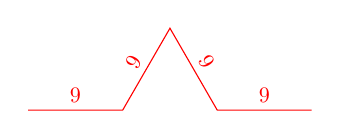
\begin{tikzpicture}[scale=0.9,every node/.style={scale=0.8}]
	\draw[red] (0,0)
			--++ (0:\Ldeux)
			node[midway,above,sloped]{9} --++ (60:\Ldeux)
			node[midway,above,sloped]{9} --++ (-60:\Ldeux)
			node[midway,above,sloped]{9} --++ (0:\Ldeux)
			node[midway,above,sloped]{9};
\end{tikzpicture}
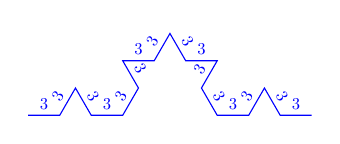
\begin{tikzpicture}[scale=0.9,every node/.style={scale=0.6}]
	\draw[blue] (0,0)
		--++ (0:\Ltrois)
		node[midway,above,sloped]{3} --++ (60:\Ltrois)
		node[midway,above,sloped]{3} --++ (-60:\Ltrois)
		node[midway,above,sloped]{3} --++ (0:\Ltrois)
		node[midway,above,sloped]{3} 
				
		--++ (60:\Ltrois)
		node[midway,above,sloped]{3} --++ (120:\Ltrois)
		node[midway,above,sloped]{3} --++ (0:\Ltrois)
		node[midway,above,sloped]{3} --++ (60:\Ltrois)
		node[midway,above,sloped]{3} 
				
		--++ (-60:\Ltrois)
		node[midway,above,sloped]{3} --++ (0:\Ltrois)
		node[midway,above,sloped]{3} --++ (-120:\Ltrois)
		node[midway,above,sloped]{3} --++ (-60:\Ltrois)
		node[midway,above,sloped]{3} 
				
		--++ (0:\Ltrois)
		node[midway,above,sloped]{3} --++ (60:\Ltrois)
		node[midway,above,sloped]{3} --++ (-60:\Ltrois)
		node[midway,above,sloped]{3} --++ (0:\Ltrois)
		node[midway,above,sloped]{3};
\end{tikzpicture}\\
	Il y a donc $4~\times~4~=~16$~segments, chacun de longueur $\dfrac{l}{3} \times \dfrac{1}{3} = \dfrac{l}{9}$. La longueur totale est $16 \times \dfrac{l}{9}$.\\
	Exemple avec $l = 27$ : longueur de la ligne $= 16 \times \dfrac{27}{9} = 16 \times 3 = 48$.

	\hrulefill
	
	On a vu avec $l = 27$\\
	Longueur du segment initial : $27$\\
	Longueur à l'étape 1 : $\left( 4 \right) \times \left( \dfrac{27}{3} \right) = 4 \times 9 = 36$\\
	Longueur à l'étape 2 : $\left( 4 \times 4 \right) \times \left( \dfrac{27}{3} \times \dfrac{1}{3} \right)
		= \left( 4 \times 4 \right) \times \left( 9 \times \dfrac{1}{3} \right)
		= 16 \times 3
		= 48$
		
	\hrulefill	


	\item Peut-on prévoir l'évolution de la longueur si on continue le processus une troisième~fois~? une quatrième fois~? \ldots une centième fois ?\\
	La longueur est le produit suivant~:  \og nombre de segments\fg{} $\times$ \og leur longueur respective\fg{}. On remarque qu'à l'étape précédente on a~: $16 \times \dfrac{l}{9}$ c'est-à-dire $16$~segments de longueur $\dfrac{l}{9}$ soit $16 \times \dfrac{l}{9}$ que l'on peut écrire $\underbrace{\left( 4 \times 4 \right)}_{\text{Nombre de segments à cette étape}} \times \underbrace{\left(\dfrac{l}{3} \times \dfrac{1}{3}\right)}_{\text{Longueur d'un segment à cette étape}}$.\\[2em]
	Longueur du segment initial : $l$\\
	Longueur à l'étape 1 : $\left( 4 \right) \times \left( \dfrac{l}{3} \right)$\\
	Longueur à l'étape 2 : $\left( 4 \times 4 \right) \times \left( \dfrac{l}{3} \times \dfrac{1}{3} \right)$\\
	Longueur à l'étape 3 : $\left( 4 \times 4 \times \ldots \right) \times \left( \dfrac{l}{3} \times \dfrac{1}{3} \times \ldots \right)$\\
	Longueur à l'étape \ldots : $\left( 4 \times 4 \times \ldots \ldots \ldots \right) \times \left( \dfrac{l}{3} \times \dfrac{1}{3} \times \ldots \ldots \ldots \right)$\\
	\vdots\\[1em]

	Et maintenant, pouvez-vous exprimer la longueur aux étapes suivantes~?\\
	Pouvez-vous la calculer~?\\[2em]
	
\end{enumerate}